\subsection{Dữ liệu: Số biến - Đa biến}
\textit{TimeWheel} [417] là một kỹ thuật để trực quan hóa nhiều biến phụ thuộc thời gian. TimeWheel bao gồm một trục thời gian và nhiều trục cho các biến dữ liệu khác. Trục thời gian được đặt ở trung tâm của hình vẽ để nhấn mạnh đặc tính thời gian của dữ liệu. Các trục của biến dữ liệu khác được ánh xạ bởi các màu khác nhau và dược sắp xếp theo hình tròn quanh trục thời gian. Để trực quan hóa dữ liệu, các đường tỏa ra từ trục thời gian đến mỗi trục khác thiết lập một kết nối giữa thời điểm và các giá trị dữ liệu liên quan. Những đường này tạo thành các nhịp điệu để người dùng xác định mối tương quan với trục thời gian, xu hướng hoặc ngoại lai. Mỗi mẫu như vậy có thể được phân biệt một cách rõ nhất với các trục song song với trục thời gian. Để tập trung vào trục mong muốn, người dùng có thể xoay TimeWheel. Các trục được tập trung có thể được nhấn mạnh bằng cách kéo dài ra. Các trục vuông góc với trục thời gian thì khó giải thích hơn, vì thế  chúng được làm nhạt bớt màu đi và co lại. Khám phá tương tác, bao gồm điều hướng trong thời gian được hỗ trợ thông qua các trục tương tác khác nhau.
\begin{figure}[H] % places figure environment here   
    \centering % Centers Graphic
    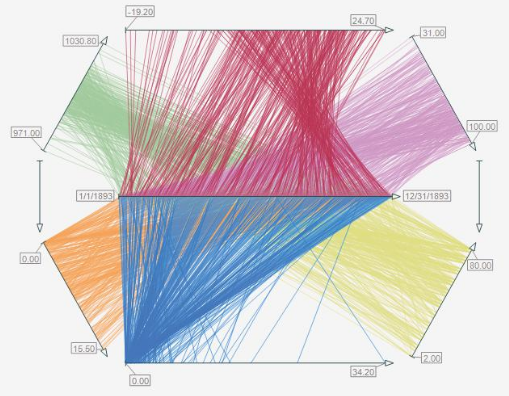
\includegraphics[width=0.8\textwidth]{assets/fig_7_7.png} 
    \caption{Trung tâm của TimeWheel [417] là trục thể hiện thời gian. Các trục khác thể hiện các biến phụ thuộc vào thời gian, hình này thể hiện 8 biến khác nhau tương ứng với 8 trục. Ở giữa, các đường đỏ thể hiện nhiệt độ trung bình, nó tăng khi bắt đầu và giảm về cuối trục thời gian. Các đường xanh dương là lượng mưa. Có một vài ngoại lại với lượng mưa cao nhưng lượng mưa cả năm thì không bất thường (Nguồn: VisAxes) } % Creates caption underneath graph
    \label{fig:f7.7}
\end{figure}